\jxhj{%教学后记
	}
\skrq{%授课日期
	2018年1月4日 4-5节}
\ktmq{%课题名称
	 坐标系旋转二}
\jxmb{%教学目标,每行前面要加 \item
	\item 掌握Fanuc上的坐标系旋转指令;
	\item 掌握Siemens上的坐标系旋转指令;
	\item 会使用旋转指令编程。}
\jxzd{%教学重点,每行前面要加 \item
	\item Fanuc上的坐标系旋转指令;
	\item Siemens上的坐标系旋转指令。 }
\jxnd{%教学难点,每行前面要加 \item
	\item 使用旋转指令编程。 }
\jjff{%教学方法
	通过讲述、举例、演示法来说明;}

\makeshouye %制作教案首页

%%%%教学内容
\subsection{组织教学}
\begin{enumerate}[\hspace{2em}1、]
	\item 集中学生注意力;
	\item 清查学生人数;
	\item 维持课堂纪律;
\end{enumerate}

\subsection{复习导入及主要内容}
\begin{enumerate}[1、]
\item 旋转应用情况;
\item 旋转指令的要素;
\item Fanuc指令格式;
\item Siemens指令格式。
\end{enumerate}

\subsection{教学内容及过程}
	
\subsubsection{要素及原理}
	1、旋转指令的要素:
	
	旋转平面
	
	旋转中心
	
	旋转角度
	
	2、原理:
	
	在CNC内部对目标点进行转换(我们不用管它)
	
	$X'=X*COSA+Y*SINA$
	
	$Y'=Y*COSA-X*SINA$
	
	\begin{figure}[h]
		\centering
		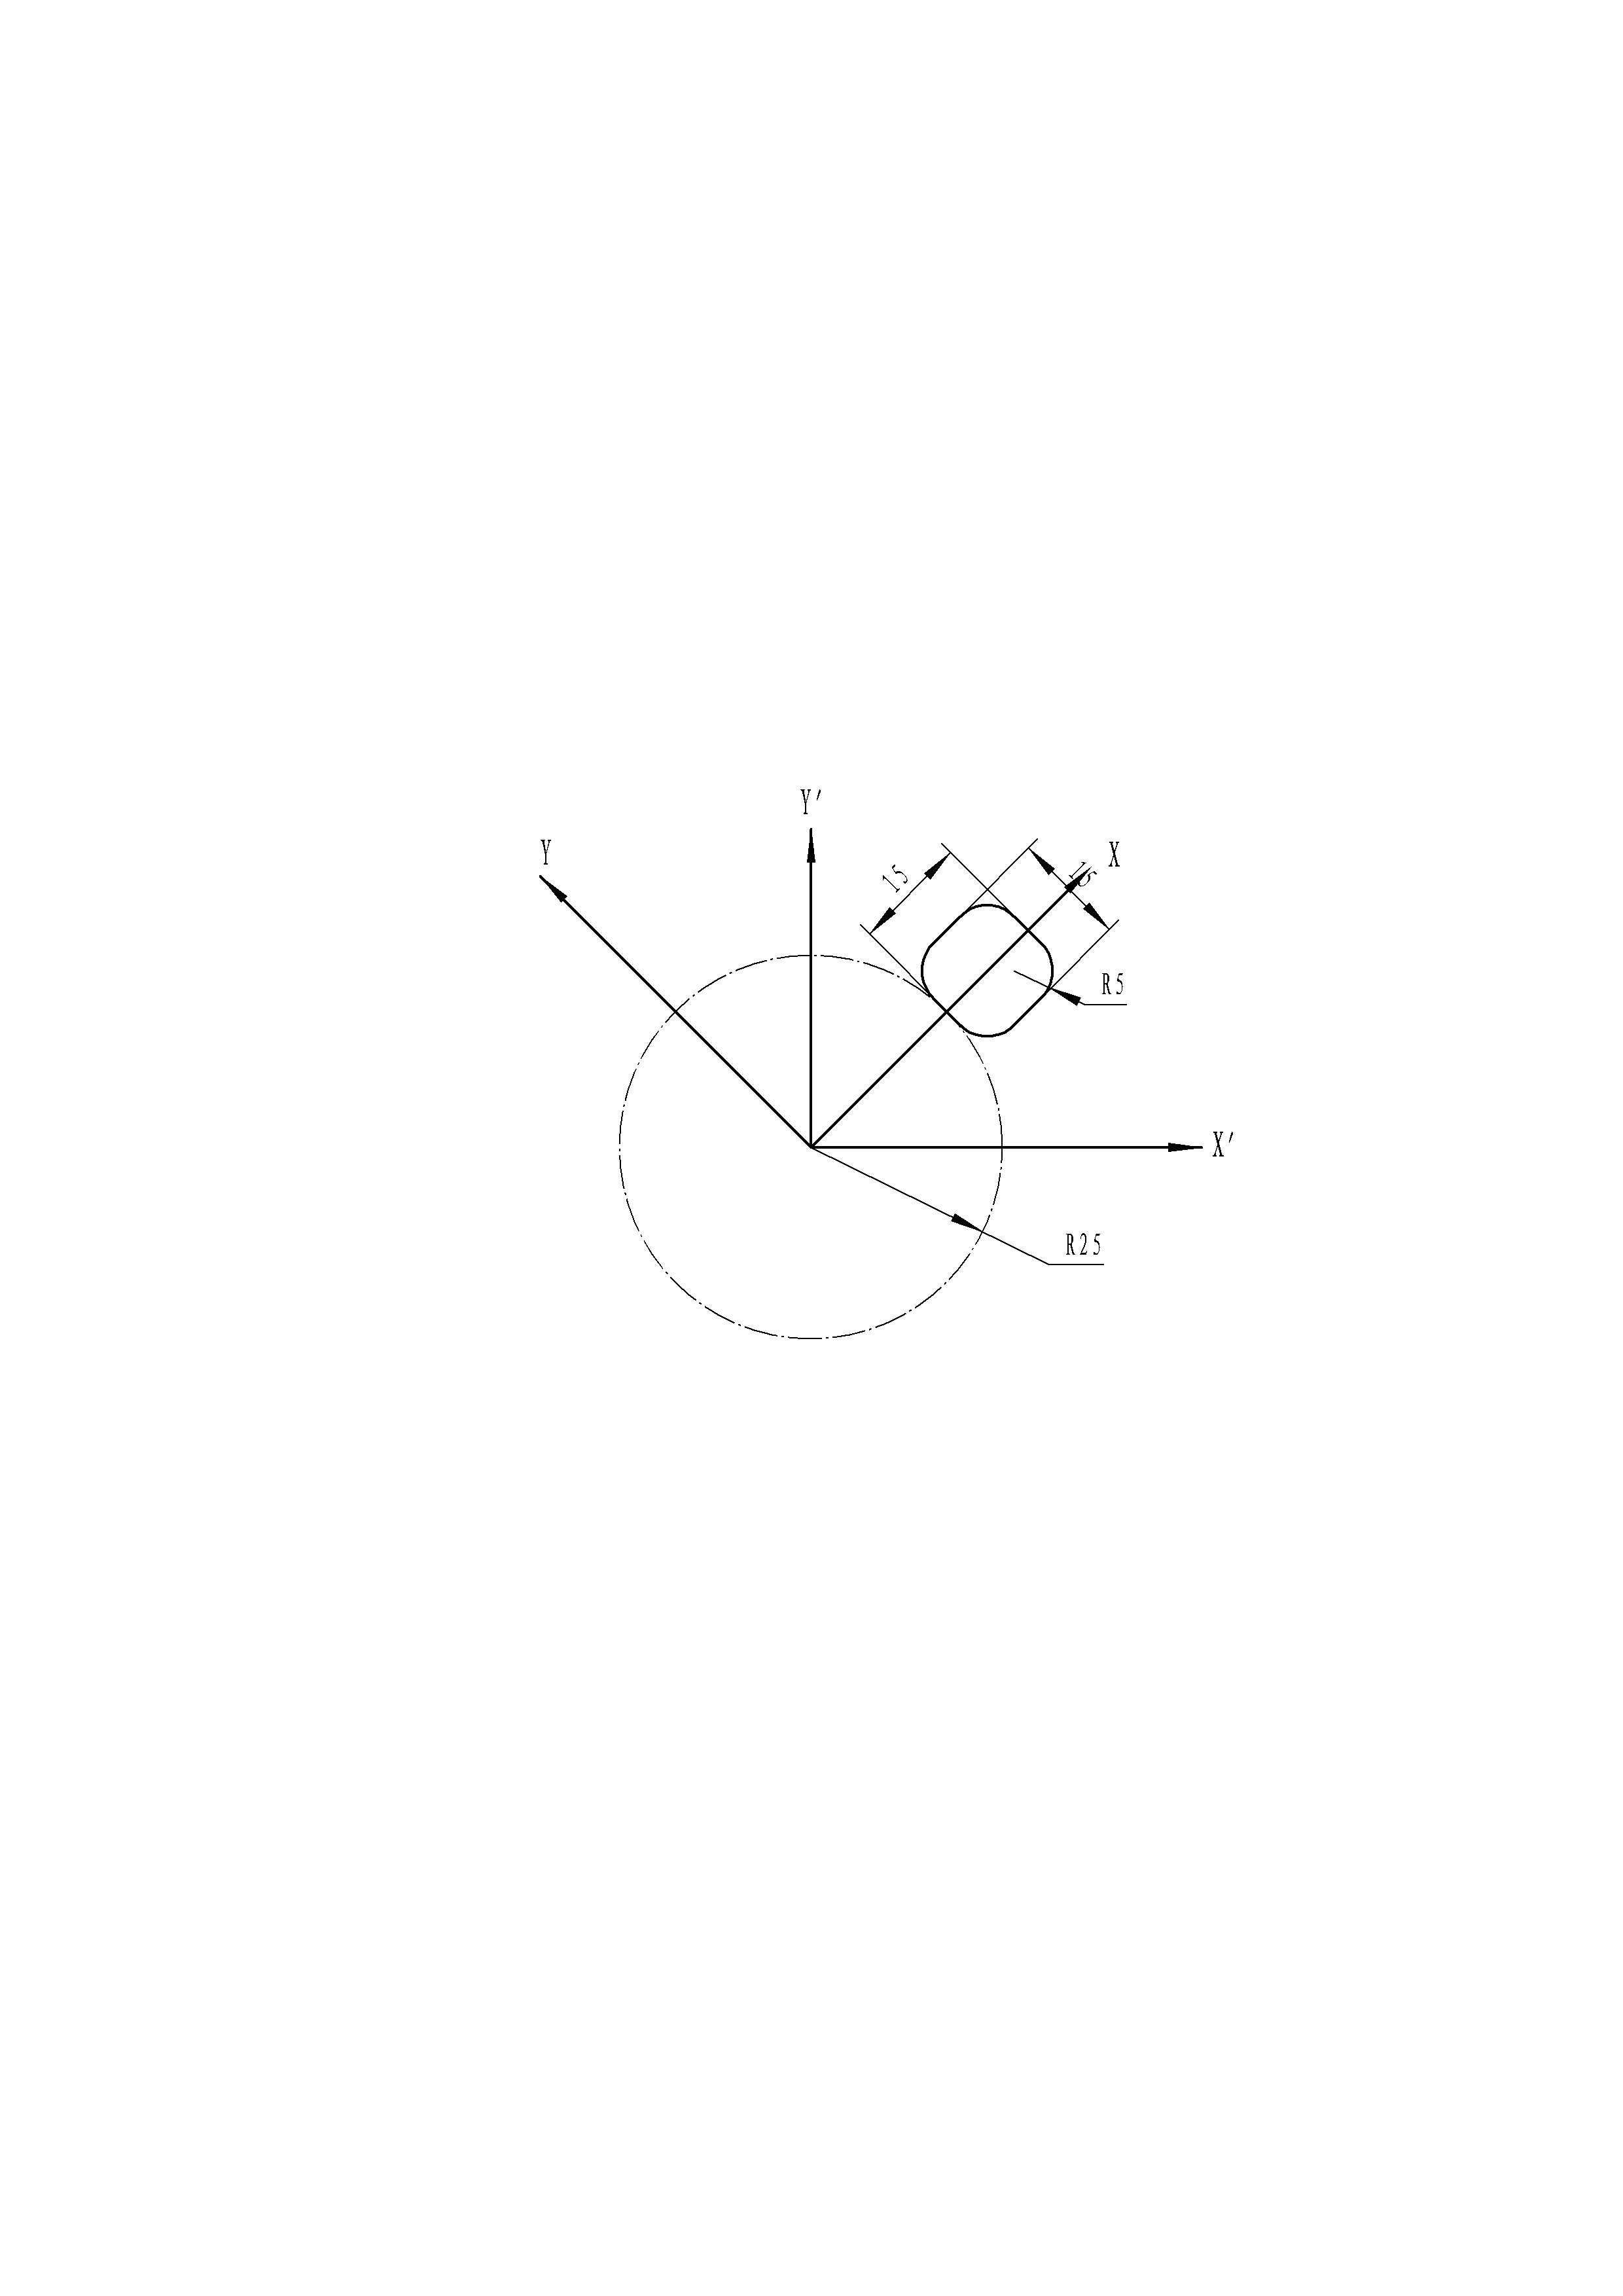
\includegraphics[width=0.7\linewidth,trim=50 285 50  250,clip]{data/image/31-1}
		\caption{原理}
		\label{fig:31-1}
	\end{figure}
	
	图中的A为-45度(即从X------X’的方向)
	
	
\subsubsection{Fanuc指令格式}

G17

G18 G68 $\alpha$\_ $\beta$\_ R\_; 坐标系旋转开始

G19

:                  坐标系旋转模式 

:                  ( 坐标系被旋转 )

G69;                坐标系旋转取消模式

说明:

G17(G18或G19): 选择包含有被旋转图形的平面

$\alpha$\_ $\beta$\_ :         对应当前平面指令(G17,G18或G19)中的两个轴的绝对指令。

此指令指定了G68后面指定旋转中心的坐标。

R\_    :         正值为逆时针方向的角度位移。参数5400Bit0指定角度位移是绝对值位移或者由G码(G90或G91)来决定绝对值或相对值。

最小输入增量: 0.001度

有效数据范围: -360.000------360.000


\subsubsection{Sienes指令格式}

功能:在当前的平面G17或G18或G19中执行旋转,值为 RPL=\_\_\_\_,单位为度。

编程:    ROT RPL=\_\_\_\_;  可编程旋转,删除以前的偏移,旋转,比例系数和镜像指令。

AROT RPL=\_\_\_\_; 可编程旋转,附加于当前的指令

ROT    没有设定值:删除以前的偏移,旋转,比例系数和镜象

ROT/AROT指令要求一个独立的程序段。

\subsubsection{加工实例}
在数控机床上加工如图所示的零件,完成加工工艺及加工程序的编写

\begin{figure}[h]
	\centering
	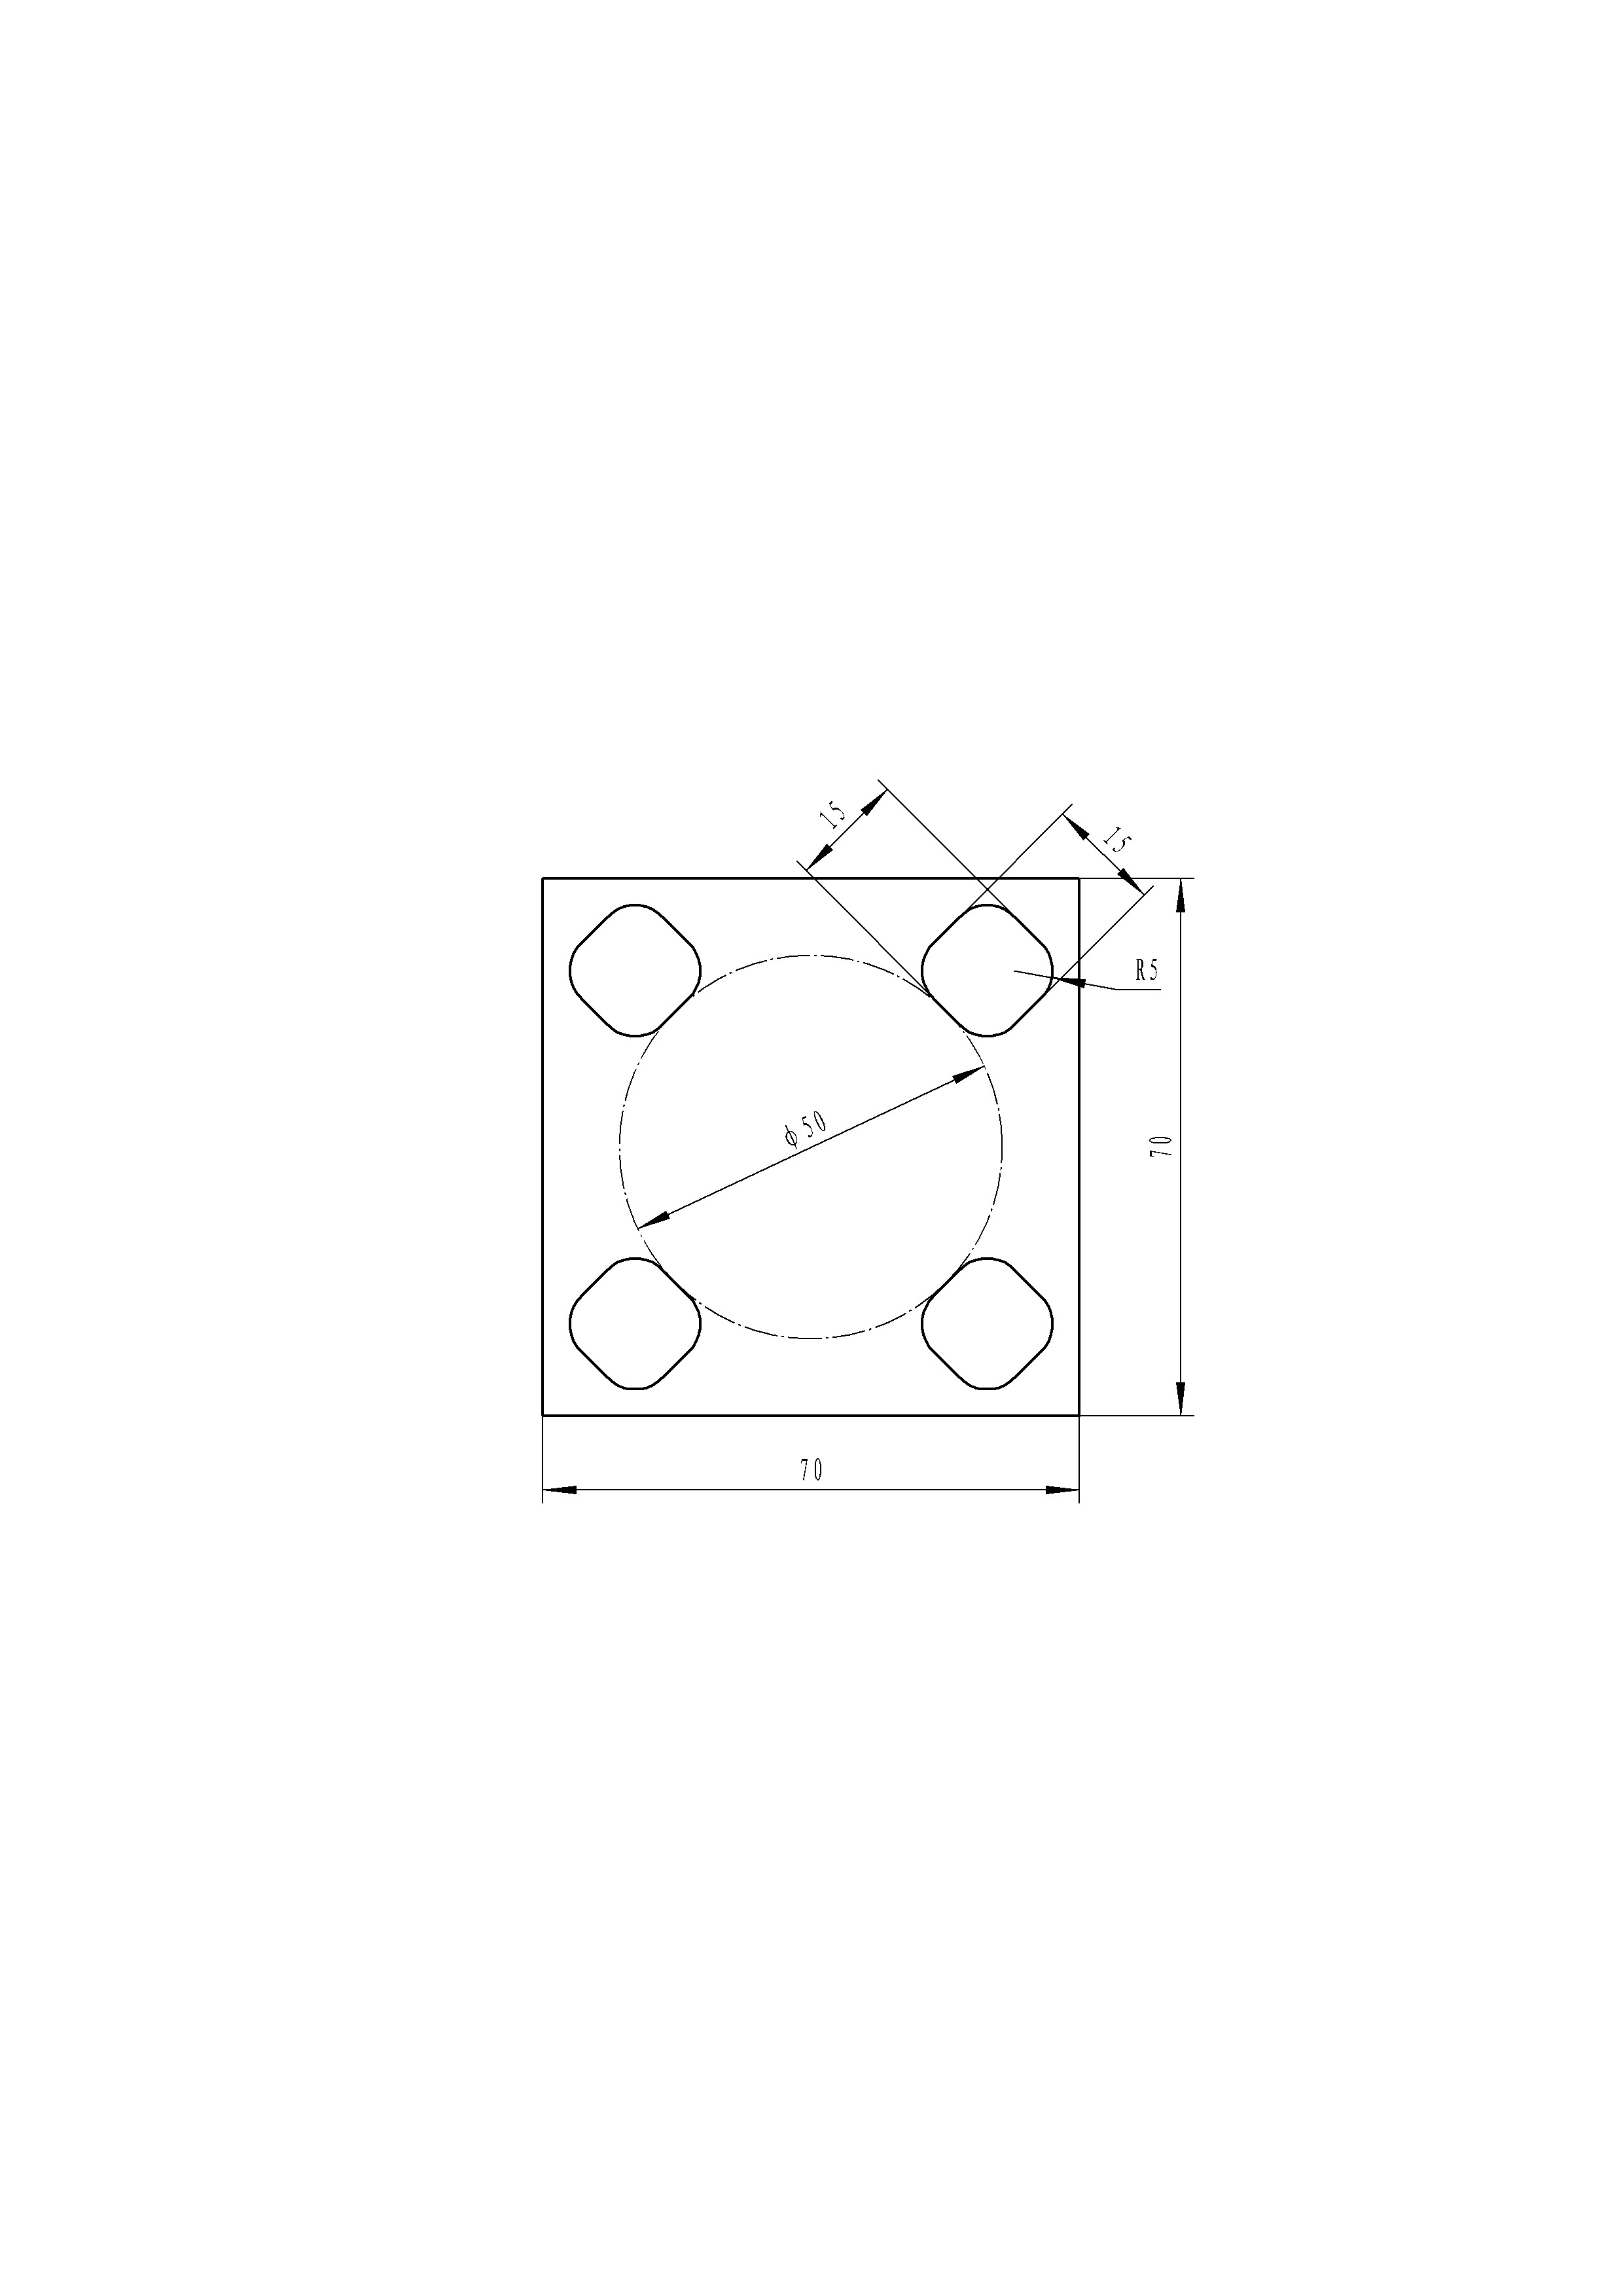
\includegraphics[width=0.7\linewidth,trim=0 0 0 0,clip]{data/image/32-1}
	\caption{加工实例}
	\label{fig:32-1}
\end{figure}

参考程序:
\begin{lstlisting}
02
G54G17G40G49G90
M3S500
G43H1G1Z100.F2000;
G1X40.Y40.
Z5.0
Z0F2000
G68X0Y0R45.
M98P221
G69
.
.
.

\end{lstlisting}

\subsection{课堂小结}
\begin{enumerate}[1、]
\item Fanuc指令格式;
\item Sienes指令格式;
\item 编程实例。
\end{enumerate}

\vfill
\subsection{布置作业}
\begin{enumerate}[1、]
	\item 综合习题一。
\end{enumerate}
\vfill